\section{Computer Vision}

The computer vision subsystem is a software component that is designed to recognise and track vehicles in images in order to count them and estimate their speed, henceforth to be referred to as the \emph{detection} component of the system. Each time an image is processed by the detection algorithm several subprocesses are performed in order to manipulate the original image into a state where vehicles have been isolated. These subprocesses can be seen in Figure \ref{fig:detection_design}. The vehicle tracking subprocess was largely influenced by the work of Adrian Rosebrock \cite{adrian_rosebrock_simple_object_tracking}\cite{adrian_rosebrock_vehicle_tracking} of PyImageSearch and the vehicle segmentation subprocess was influenced by the work of Andrey Nikishaev \cite{andrey_nikishaev_traffic_counting}. Much of the functionality is provided by the Python open source computer vision library, OpenCV \cite{opencv}


\begin{figure}[H]
    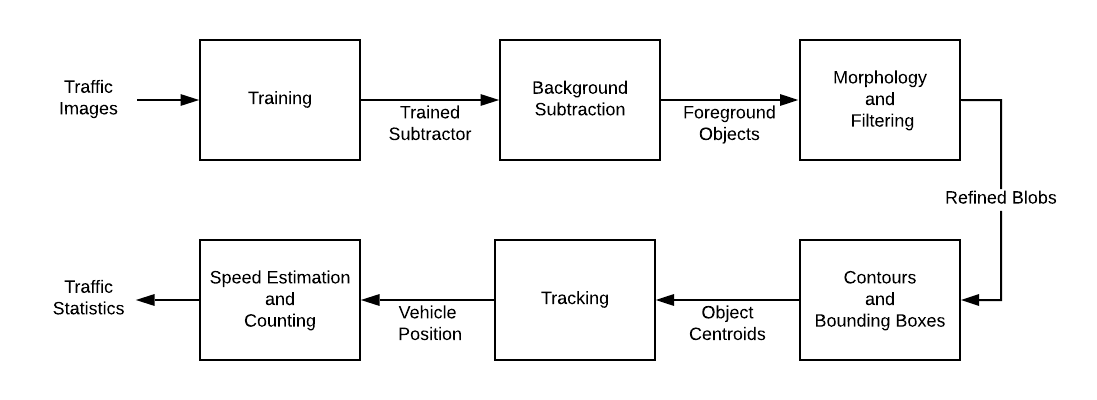
\includegraphics[width=0.9\columnwidth]{detection_design}
    \caption{Subprocess that comprise the detection subsystem.}
    \label{fig:detection_design}
\end{figure}


\subsection{Training}
\label{subsection:training}
The training component of the detection subsystem occurs only once at the initialization of the system. It's purpose is to 'train' a subtractor algorithm (section \ref{subsection:subtractor}) on what pixels of the image are probably the background. 





\subsection{Background Subtraction}
\label{subsection:subtractor}

The background subtractor function is to determine what pixels of an image are from the background and what pixels belong to objects.


\subsection{Morhpology and Filtering}

Perform some postprocessing on the output of the background subtractor. The purpose of this post processing is to modify the foreground objects presented and remove and spurious entities that either are not objects in the first place or are too small to be represent a vehicle.


\subsection{Countours and Bounding Boxes}

Contours represent the outline of a foreground object and bounding boxes are the corrected squares that are placed around the polygons that represent an object's outline. These bounding boxes are important for in the tracking of a object.


\subsection{Tracking}

Tracking is follows an objects movement across multiple images. This requires that the object be reidentified in each new image and matched to it's old location.

\subsection{Speed Estimation and Counting}

This subprocess consolidates the efforts of the former ones and convert the information about an objects position into vehicle counts and speeds.